\documentclass[11pt, a4paper]{pancake-article}

\usepackage{mathtools}

\usepackage{graphicx}
\usepackage{booktabs, csvsimple}

\usepackage[
	style=apa
]{biblatex}
\addbibresource{Bibliography.bib}

\usepackage{siunitx}
\sisetup{mode=math}

\usepackage{setspace}
\onehalfspacing

% colors!
\usepackage[usenames, dvipsnames]{xcolor}
\newcommand{\tint}[1]{{\color{accent}#1}}

\usepackage{hyperref}
\hypersetup{
	hidelinks,
	colorlinks,
	breaklinks=true,
	urlcolor=accent,
	citecolor=accent,
	linkcolor=accent,
	bookmarksopen=false,
	pdftitle={Sorting sentiments of hotel reviews through machine learning},
	pdfauthor={Darren Yap},
}

\title{Sorting \tint{sentiments} of hotel reviews through \tint{machine learning}}
\author{\tint{Yap} Hao Ming Darren \and \tint{Tan} Jia He \and \tint{Fu} Jinghang}
\date{\scshape Singapore Mathematics Project Festival 2024}

% start the document!
\begin{document}

\maketitle
\thispagestyle{empty}
\pagebreak
\tableofcontents
\thispagestyle{empty}

\pagebreak
\thispagestyle{empty}

% ** abstract **
\begin{abstract}
	Hotels depend on tourists to survive. They gather consumer opinions via customer
	reviews to improve their services. This project used sentiment analysis---the
	process of determining the emotional tone of text---to quantify consumers'
	opinions on hotels, and predicted the overall sentiment of hotel reviews.
	International hotel reviews in English were split into individual words,
	assigning each word a score based on its relative intensity. The sentiment
	makeup of the review dataset was highlighted and the most frequent tokens were
	identified. Two machine learning models---a logistic regression model and a random
	forest classifier---were also constructed to predict the overall sentiment of a
	review. It was shown that the models were capable of predicting the overall
	sentiment of hotel reviews. This project highlights the possibility of using
	sentiment analysis models to create applications that allow customers to better
	understand the perceived quality of a hotel and potentially combat review fraud---the
	the dishonest practice of manipulating false reviews to boost a hotel's ratings.
\end{abstract}

\pagebreak

\pagestyle{fancy}
\setcounter{page}{1}

\section{Introduction}
After the Singapore government relaxed travel restrictions due to COVID-19,
there has been a recent increase in the number of tourists travelling in and out of Singapore.
As such, hotels have seen a rise in the number of prospective tourists to be housed,
and this may encourage an increase in the number of reviews hotels may receive.

Today, it is common to use social networks, messengers, and review websites
to receive data from customer opinions. This is especially true for hotels,
where previous occupants may evaluate the hotel on several factors through their
reviews---be it cleanliness, facilities, location and convenience, etc.
These come in two forms---a quantitative review (based on stars, diamonds,
hearts, etc.) and a more qualitative review through text.

However, quantitative reviews do not always paint the full picture of customers'
opinions towards a certain hotel. Though it is certainly helpful to have a more
objective rating system using numerical scores, eg. the Department of Tourism
grading system in the Philippines, or the European \textit{Hotelstars} Union system,
these are given by customers subjectively and do not reflect the reasons for
customers giving the rating. There is also evidence of manipulation of ratings
by hotel management itself, where hotels may be compelled to forge positive or
negative ratings to bias the overall rating. This made up \qty{2.1}{\percent}
of the 66 million reviews submitted to TripAdvisor in 2019 (\cite{tripadvisor}).
Therefore, we propose using sentiment analysis to extract customers' true
feedback on hotels instead.

\section{Research Questions and Hypotheses}
The following were investigated, in increasing order of difficulty:
\begin{enumerate}
	\item How could the sentiments of individual words be quantified on a numerical scale?
	\item How could the sentiments of paragraphs be quantified on a numerical scale?
	\item How could tokens in hotel reviews be used to predict the overall sentiment of the review?
\end{enumerate}

The objectives of this research were as such:
\begin{enumerate}
	\item To run sentiment analysis on individual words and quantify them on a numerical scale
	\item To run sentiment analysis on paragraphs and quantify them on a numerical scale
	\item To use sentiment analysis on hotel reviews to determine consumers' overall opinions of hotels
\end{enumerate}

\section{Literature Review}
Sentiment analysis is a field of study which utilises computational methods to analyse text,
and then determine the underlying emotion it contains; at simple levels, text can be classified
into positive and negative polarities; at more complex levels, more specific emotions, such as
\textit{happy}, \textit{sad} and \textit{angry}, can be determined. It
has broad applications which range from determining consumers' opinions in sales and product
analysis to competitor research in marketing, and even detecting public opinion in social media
monitoring. Sentiment analysis will be used in this research to analyse hotel occupants' reviews
and determine their sentiments towards them, without interference from human bias.

\citeauthor{stock} (\citeyear{stock}) predicted the stock market opinion of StockTwits communities of expert
investors. Sentiment analysis was used in a deep learning model to extract sentiment from Big Data.
A Pearson Correlation Coefficient combined the linear correlation between users' sentiment and
future stock prices, which showed that the accuracy of user sentiment was \qty{53}{\percent}. It was
concluded that convolutional neural networks could predict stock market movement based on
sentiment.

Using the social networking site Twitter, \citeauthor{twitter} (\citeyear{twitter}) determined
Filipinos' sentiment in response to the Philippine government's efforts at tackling COVID-19,
specifically the implementation of vaccination. Sentiment analysis was used to extract sentiment
from text in the English and Tagalog languages, the results from which were used to train a Naïve
Bayes model. A confusion matrix was produced, representing the model's prediction accuracy
in classifying sentiment into positive, neutral and negative categories---\qty{81.77}{\percent}.
It was concluded that sentiment analysis was sufficiently accurate to help the Philippine government
better conduct budget planning and coordinate COVID-19 efforts.

\citeauthor{spain} (\citeyear{spain}) analysed tourism quality in Spain
by extracting sentiment from reviews by Chinese tourists on the tourism
social networking sites Baidu Travel, Ctrip, Mafengwo, and Qunar.
Two sentiment analysis methods, lexicon-matching and corpus-based machine
learning methods, were used. These methods allow for the processing of
unstructured text of comparatively longer lengths. Clustered data
visualisation categorised aspects of Spanish tourism into positive
and negative groups, with the majority residing within positive sentiment.
It was concluded that sentiment analysis can be used to improve tourism
quality and sustainability decision-making.

SentiStrength, a tool for lexical sentiment analysis---sentiment analysis
done on short, low quality texts---was used to study emotions expressed
in GitHub commit comments of different open-source projects (\cite{github}).
Each word was assigned a score, then the net score for each comment was calculated.
Eacch comment was split into snippets using SentiStrength, then assigned a score by
computing the maximum and minimum scores of the sentences it contains.
Following which, the average of the positive and negative scores was taken as the
sentiment score of the entire commit. This study showed that Java projects warranted
more negative comments, and projects which had more distributed teams tended
to warrant higher positive sentiments.

In conclusion, the literature reviewed showed many possible applications
of sentiment analysis in quantifying the underlying emotion of feedback
on online platforms. Lexicon-based sentiment analysis, which assigns each
word a sentiment, then calculates a sentence's total sentiment score, can
be used, due to its simplicity in implementation, and the availability of
many open-source sentiment lexicons. In addition, sentiment categorisation
using lexicon-based sentiment analysis makes accurate predictions upwards of
\qty{70}{\percent} of the time (\cite{khoo}). SentiStrength would also be useful for
detecting sentiment from hotel reviews which are usually short in length quickly
and efficiently, facilitating the process of extracting sentiment from tourists'
reviews of hotels. Using SentiStrength for sentiment calculation is also
rather accurate, generating both positive and negative sentiments with a more
than \qty{60}{\percent} accuracy (\cite{thelwall}). Therefore, the strategies listed
above could be adopted or emulated on a smaller scale for this project.

\section{Methods and Results}

\subsection{Token-based sentiment analysis}\label{sec:tokens}
After collecting an open-source dataset of international hotel reviews in English from Datafiniti,
the reviews were tokenised and split into individual tokens. The Afinn lexicon was then obtained,
which was used to assign each token a single integer score, ranging from \(\left[-5, -1\right]\) for
negative tokens, and \(\left[1, 5\right]\) for positive ones. It was found that the vast majority
of tokens in the dataset held a positive sentiment  after a large number of neutral tokens were disregarded
(Figure~\ref{fig:bars}). The high number of neutral tokens can be attributed to nouns
describing the hotel, like \textit{food}, \textit{hotel} and \textit{pool}.

\begin{figure}[htpb]
	\centering
	\begin{minipage}{0.5\textwidth}
		\centering
		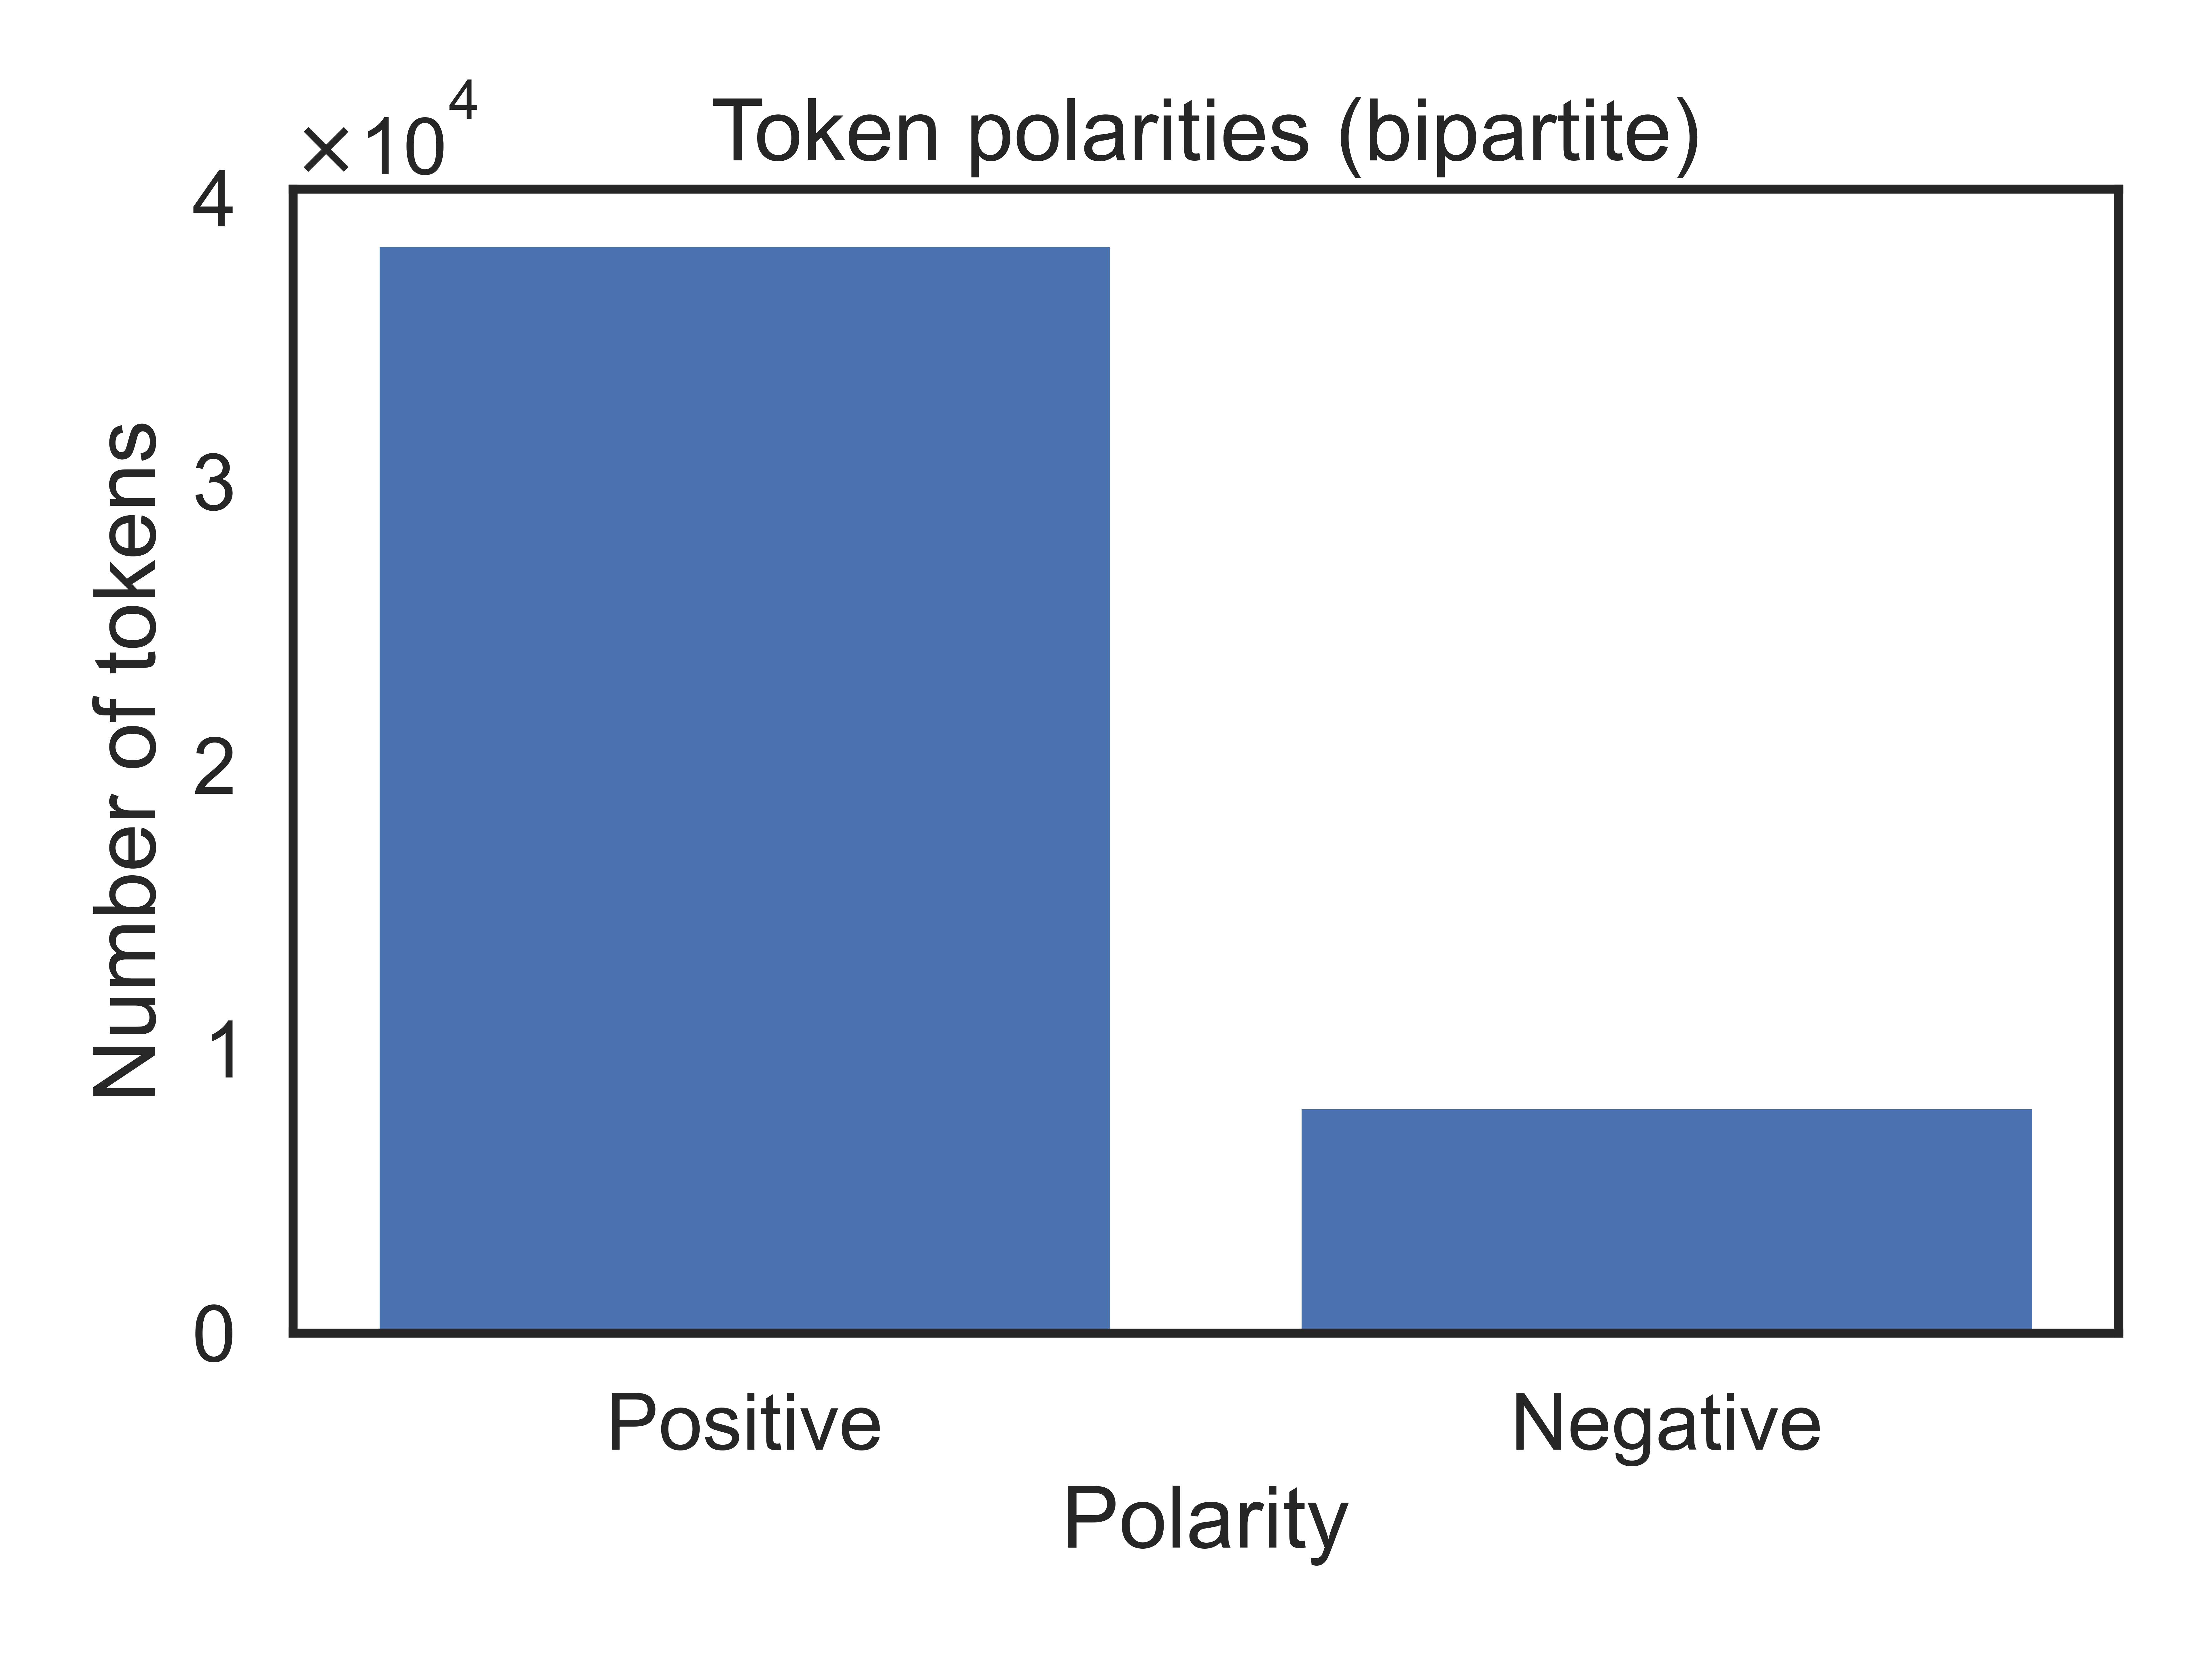
\includegraphics[width=\textwidth]{../results/old/bar_bipartite.png}
		\caption*{Bipartite sentiment}
	\end{minipage}\hfill
	\begin{minipage}{0.5\textwidth}
		\centering
		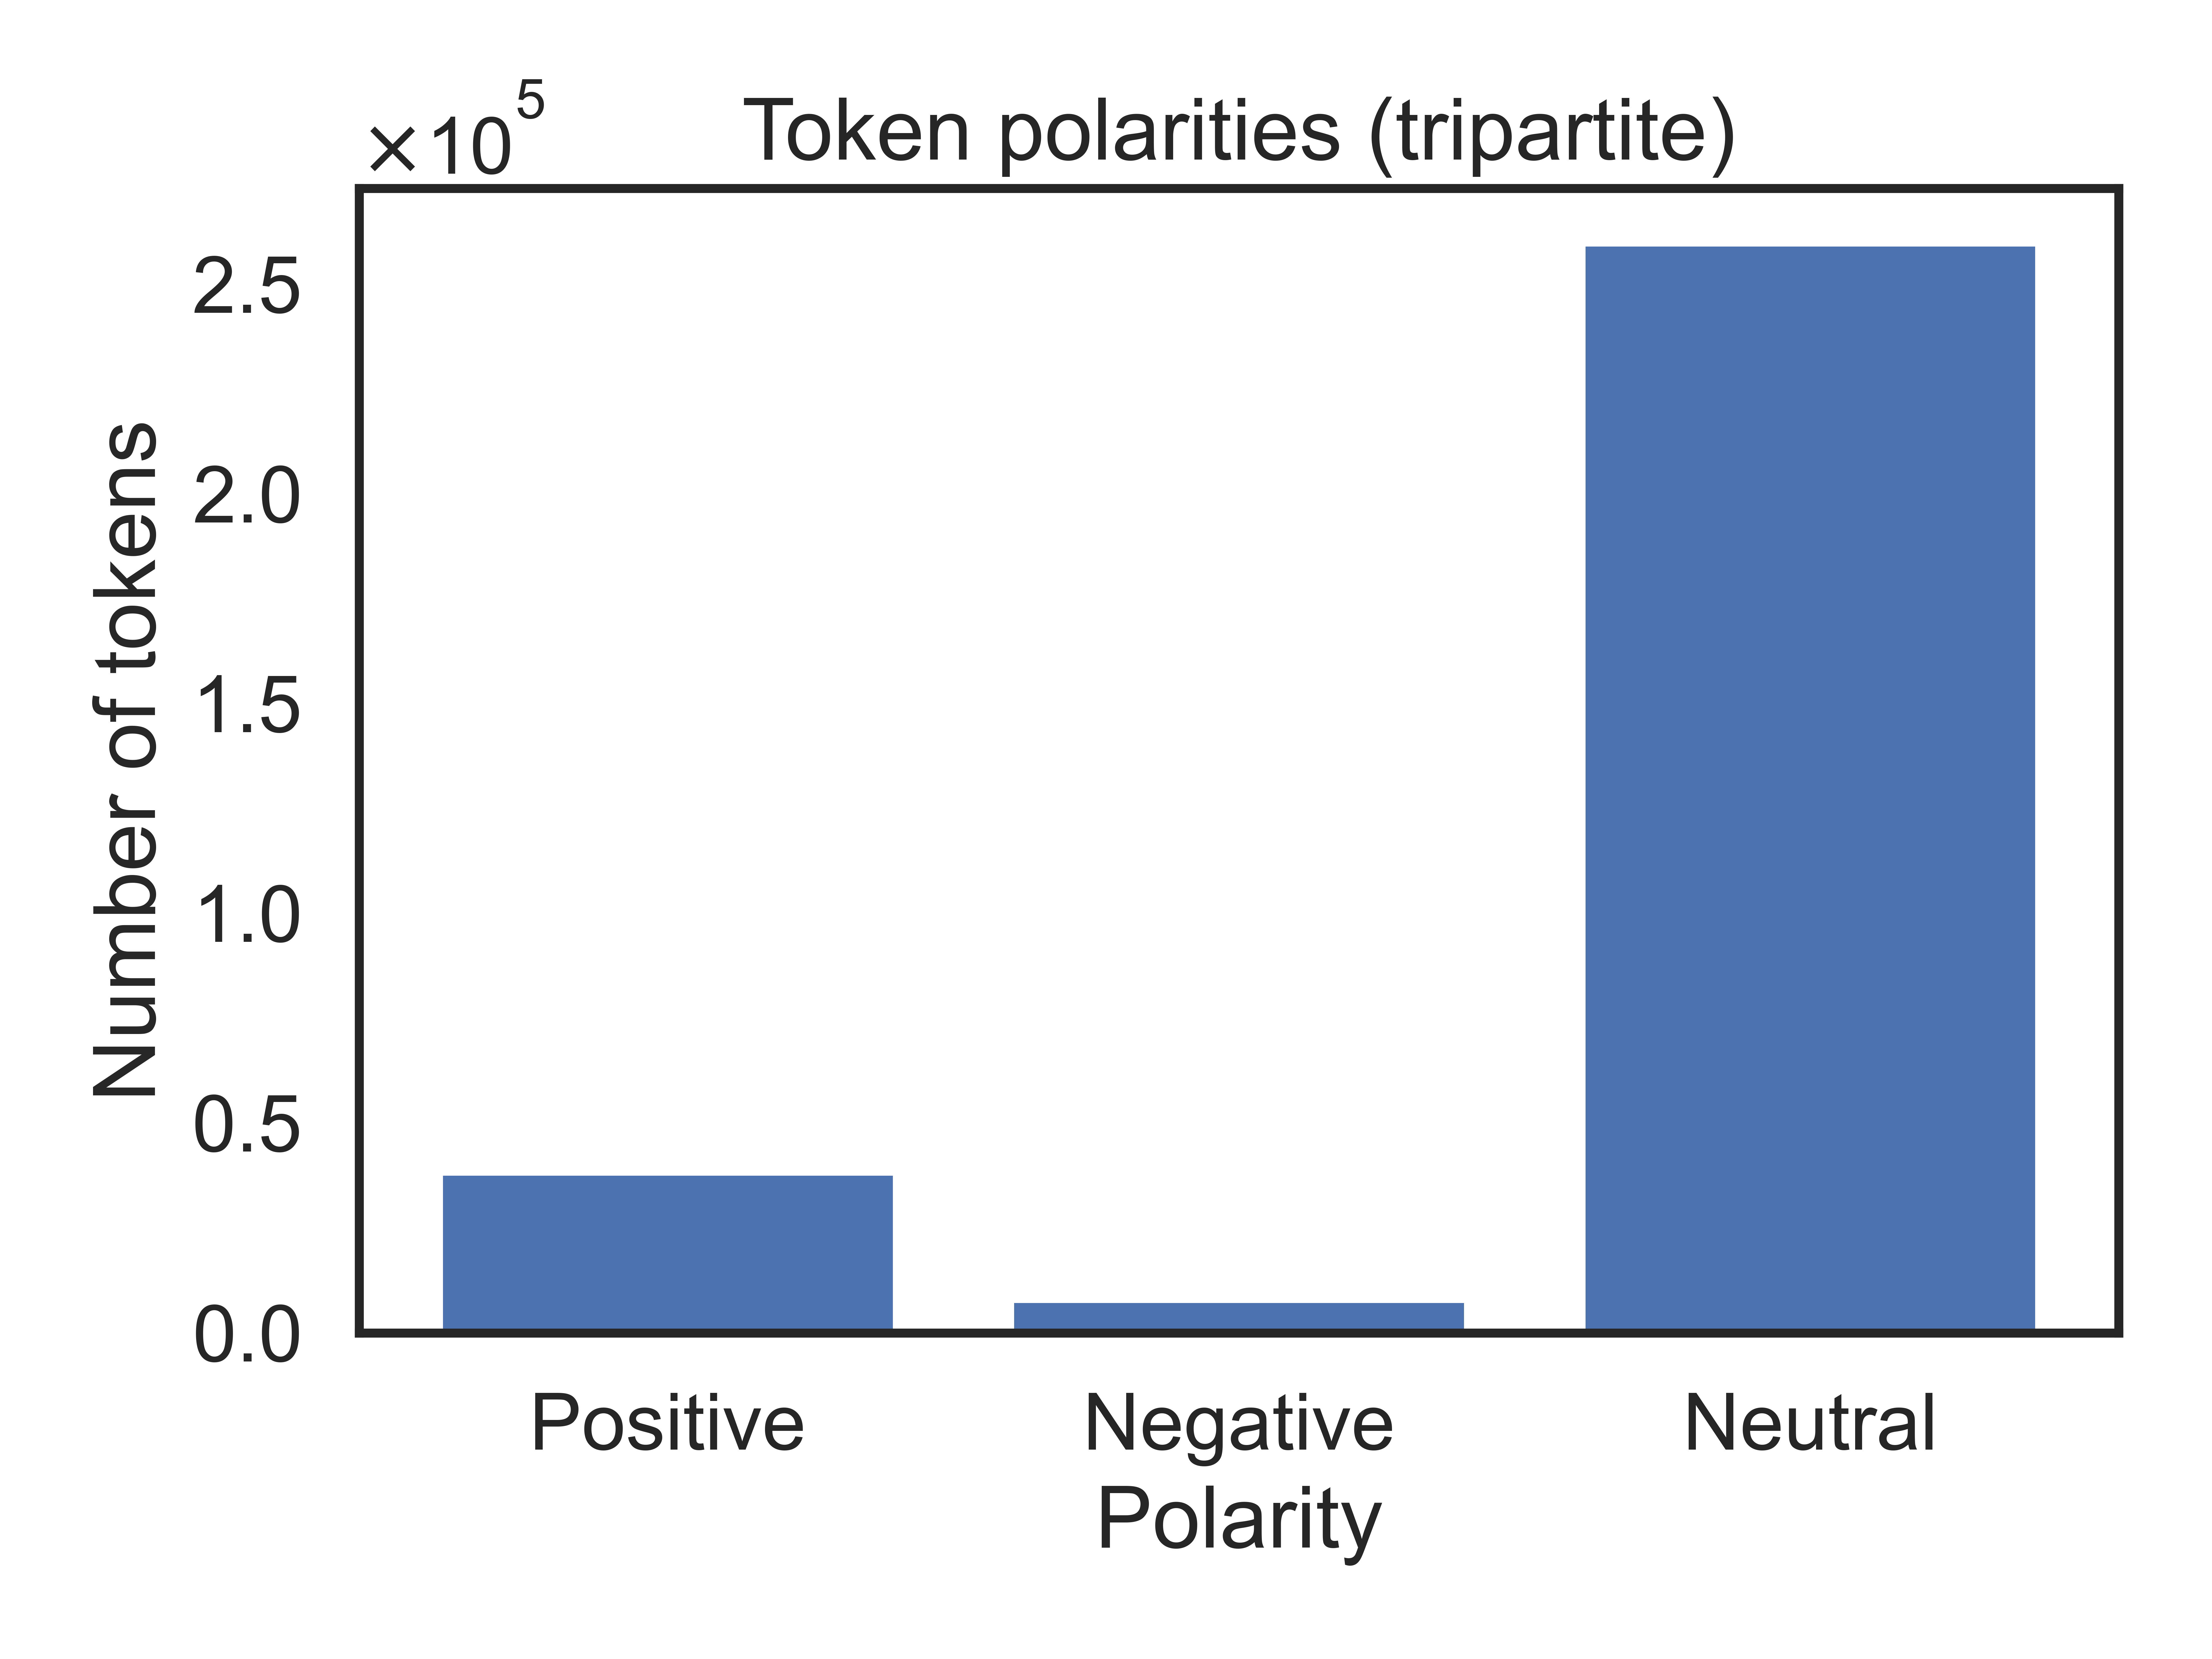
\includegraphics[width=\textwidth]{../results/old/bar_tripartite.png}
		\caption*{Tripartite sentiment}
	\end{minipage}
	\caption{Proportion of tokens by polarity}
	\label{fig:bars}
\end{figure}

It is also noted that generic tokens associated with ``goodness'' are more
prominent when discussing a hotel's desirable traits, such as \textit{great},
\textit{good} and \textit{nice}, whereas visitors were more likely to
describe the hotel in detail when criticising it, citing traits like
\textit{dirty}, \textit{noisy} and \textit{hard} (Figure~\ref{fig:wordclouds}).

\begin{figure}[htpb]
	\centering
	\begin{minipage}{0.5\textwidth}
		\centering
		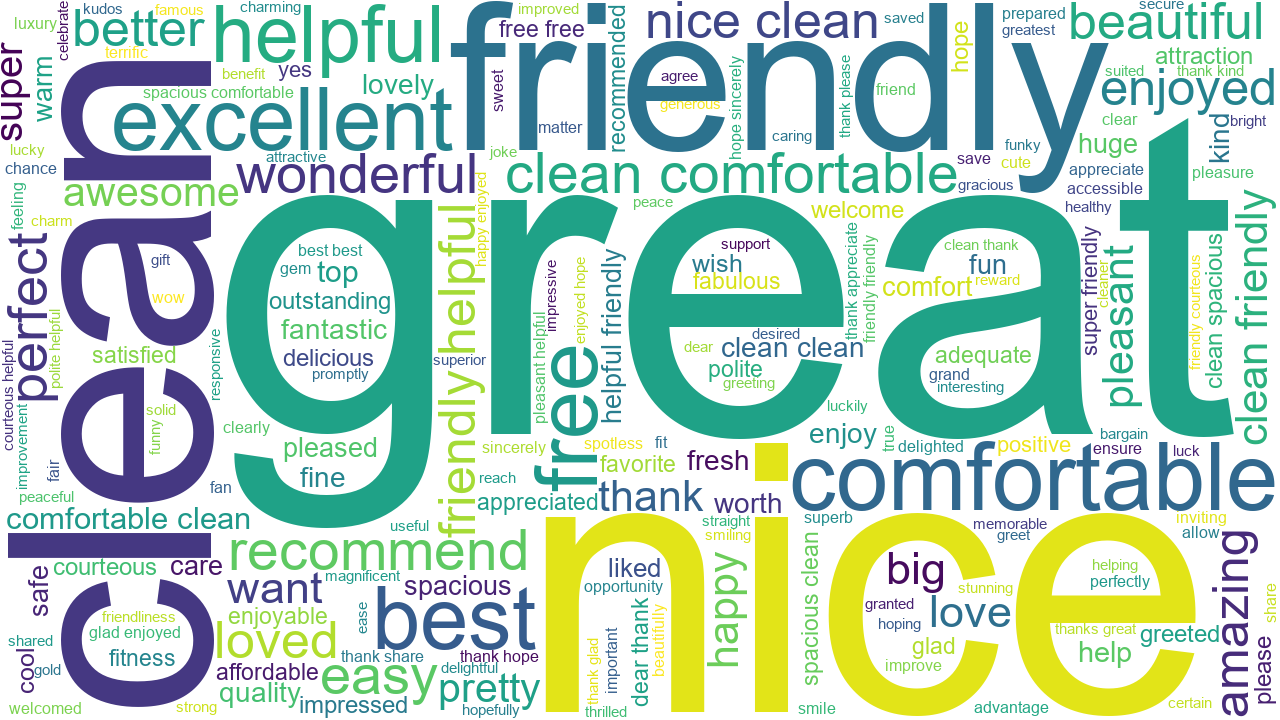
\includegraphics[width=0.9\textwidth]{../results/old/wordcloud_1.png}
		\caption*{Positive tokens}
	\end{minipage}\hfill
	\begin{minipage}{0.5\textwidth}
		\centering
		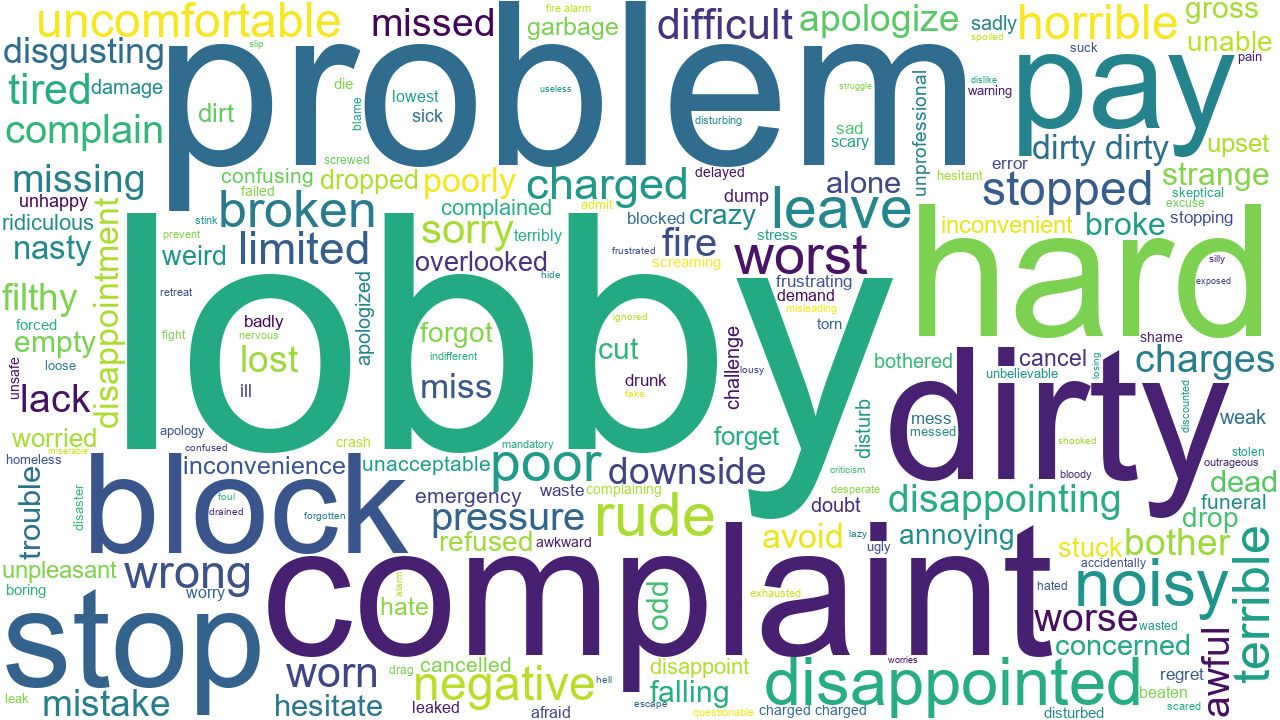
\includegraphics[width=0.9\textwidth]{../results/old/wordcloud_0.png}
		\caption*{Negative tokens}
	\end{minipage}
	\caption{Wordclouds of tokens by polarity}
	\label{fig:wordclouds}
\end{figure}

\subsection{Review-based sentiment analysis}\label{sec:reviews}

The software SentiStrength was used to generate two scores for each review:
a positive one in the range \(\left[1, 5\right]\) and a negative one in the range \(\left[–5, –1\right]\).
The greater the tonal intensity of a word, the greater the magnitude of the sentiment score
it would contribute to the overall positive or negative score of the review. Punctuation marks for
emphasis were also considered. After this, the reviews were classified into two categories: overall
positive (polarity \(1\)), and negative (polarity \(0\)). Where \(y\) is the polarity
of a review, and \(s_+\) and \(s_-\) are the positive and negative sentiment scores (Equation~\ref{eq:polarity}):

\begin{equation}
	y = \begin{cases}
		1 & s_+ + s_- \geq 0 \\
		0 & s_+ + s_- < 0    \\
	\end{cases}
	\label{eq:polarity}
\end{equation}

It is observed that a large proportion of reviews were overall positive (\qty{70}{\percent})
and only a handful of negative reviews were present (\qty{13}{\percent}) in the dataset.
Though neutral reviews may seem to make up a sizeable proportion of the reviews, this merely
shows that the magnitude of the positive and negative sentiment scores is equal (Figure~\ref{fig:pies}).

\begin{figure}[htpb]
	\centering
	\begin{minipage}{0.5\textwidth}
		\centering
		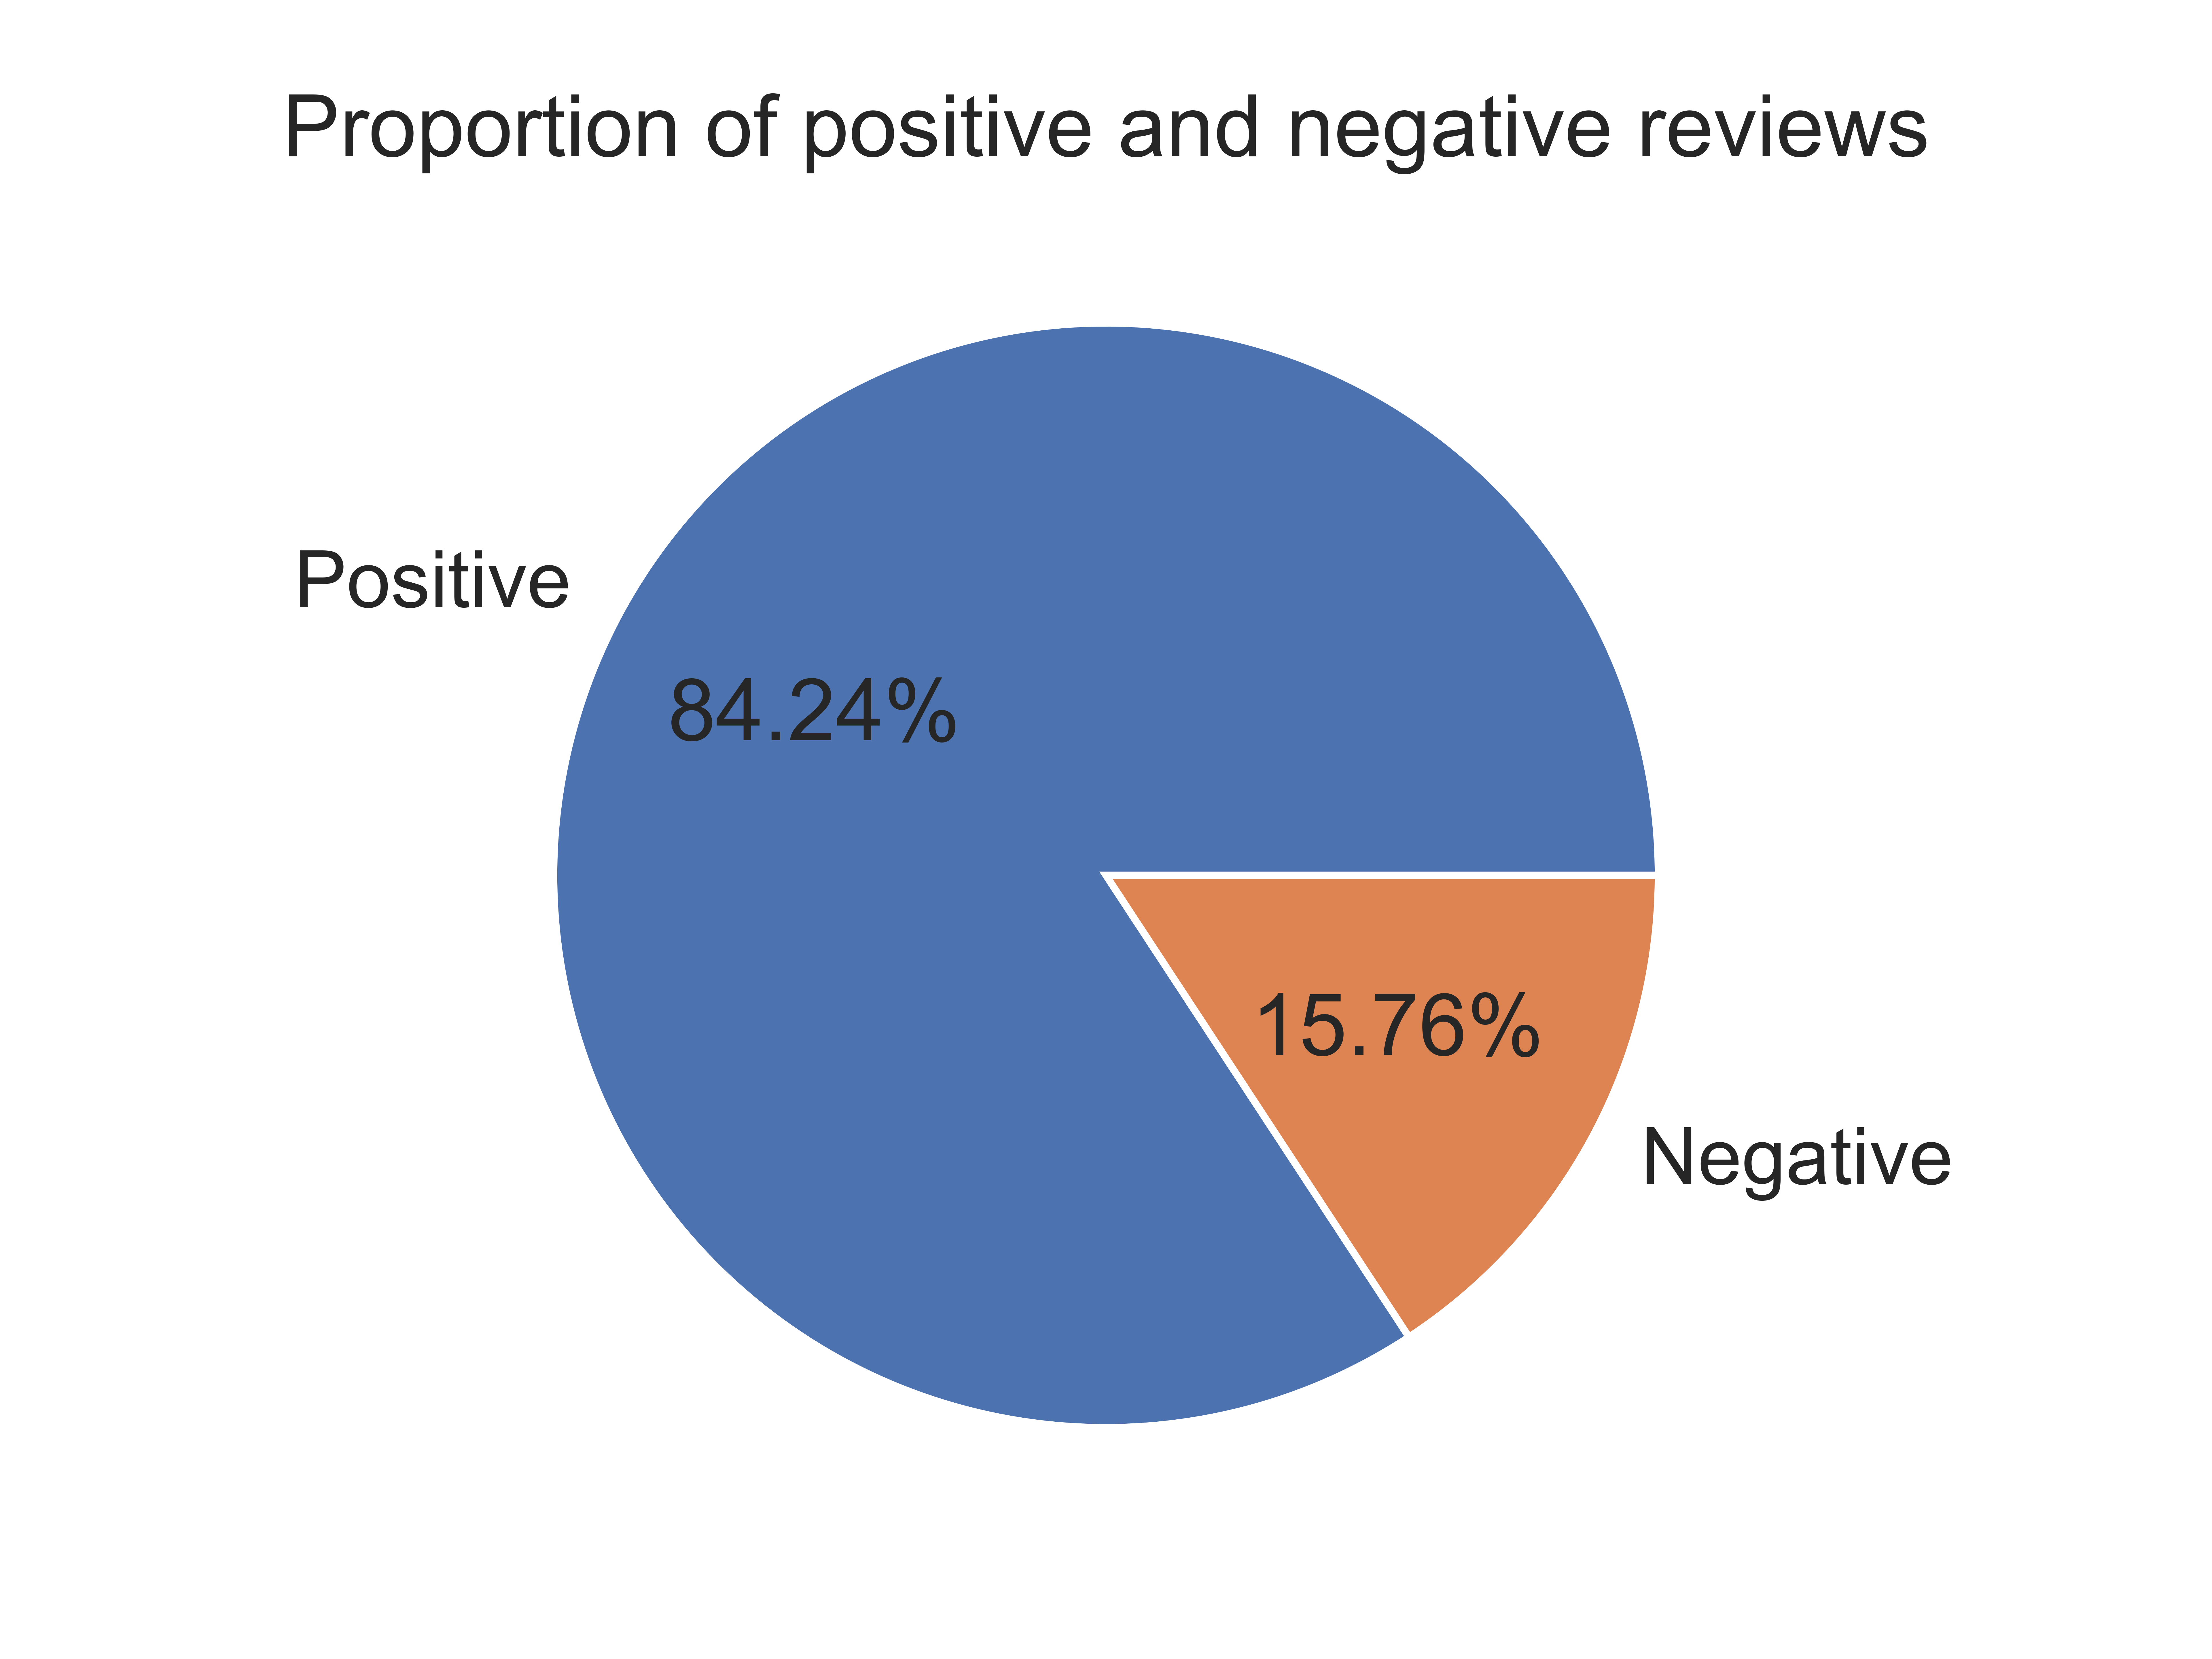
\includegraphics[width=0.9\textwidth]{../results/old/pie_bipartite.png}
		\caption*{Bipartite sentiment}
	\end{minipage}\hfill
	\begin{minipage}{0.5\textwidth}
		\centering
		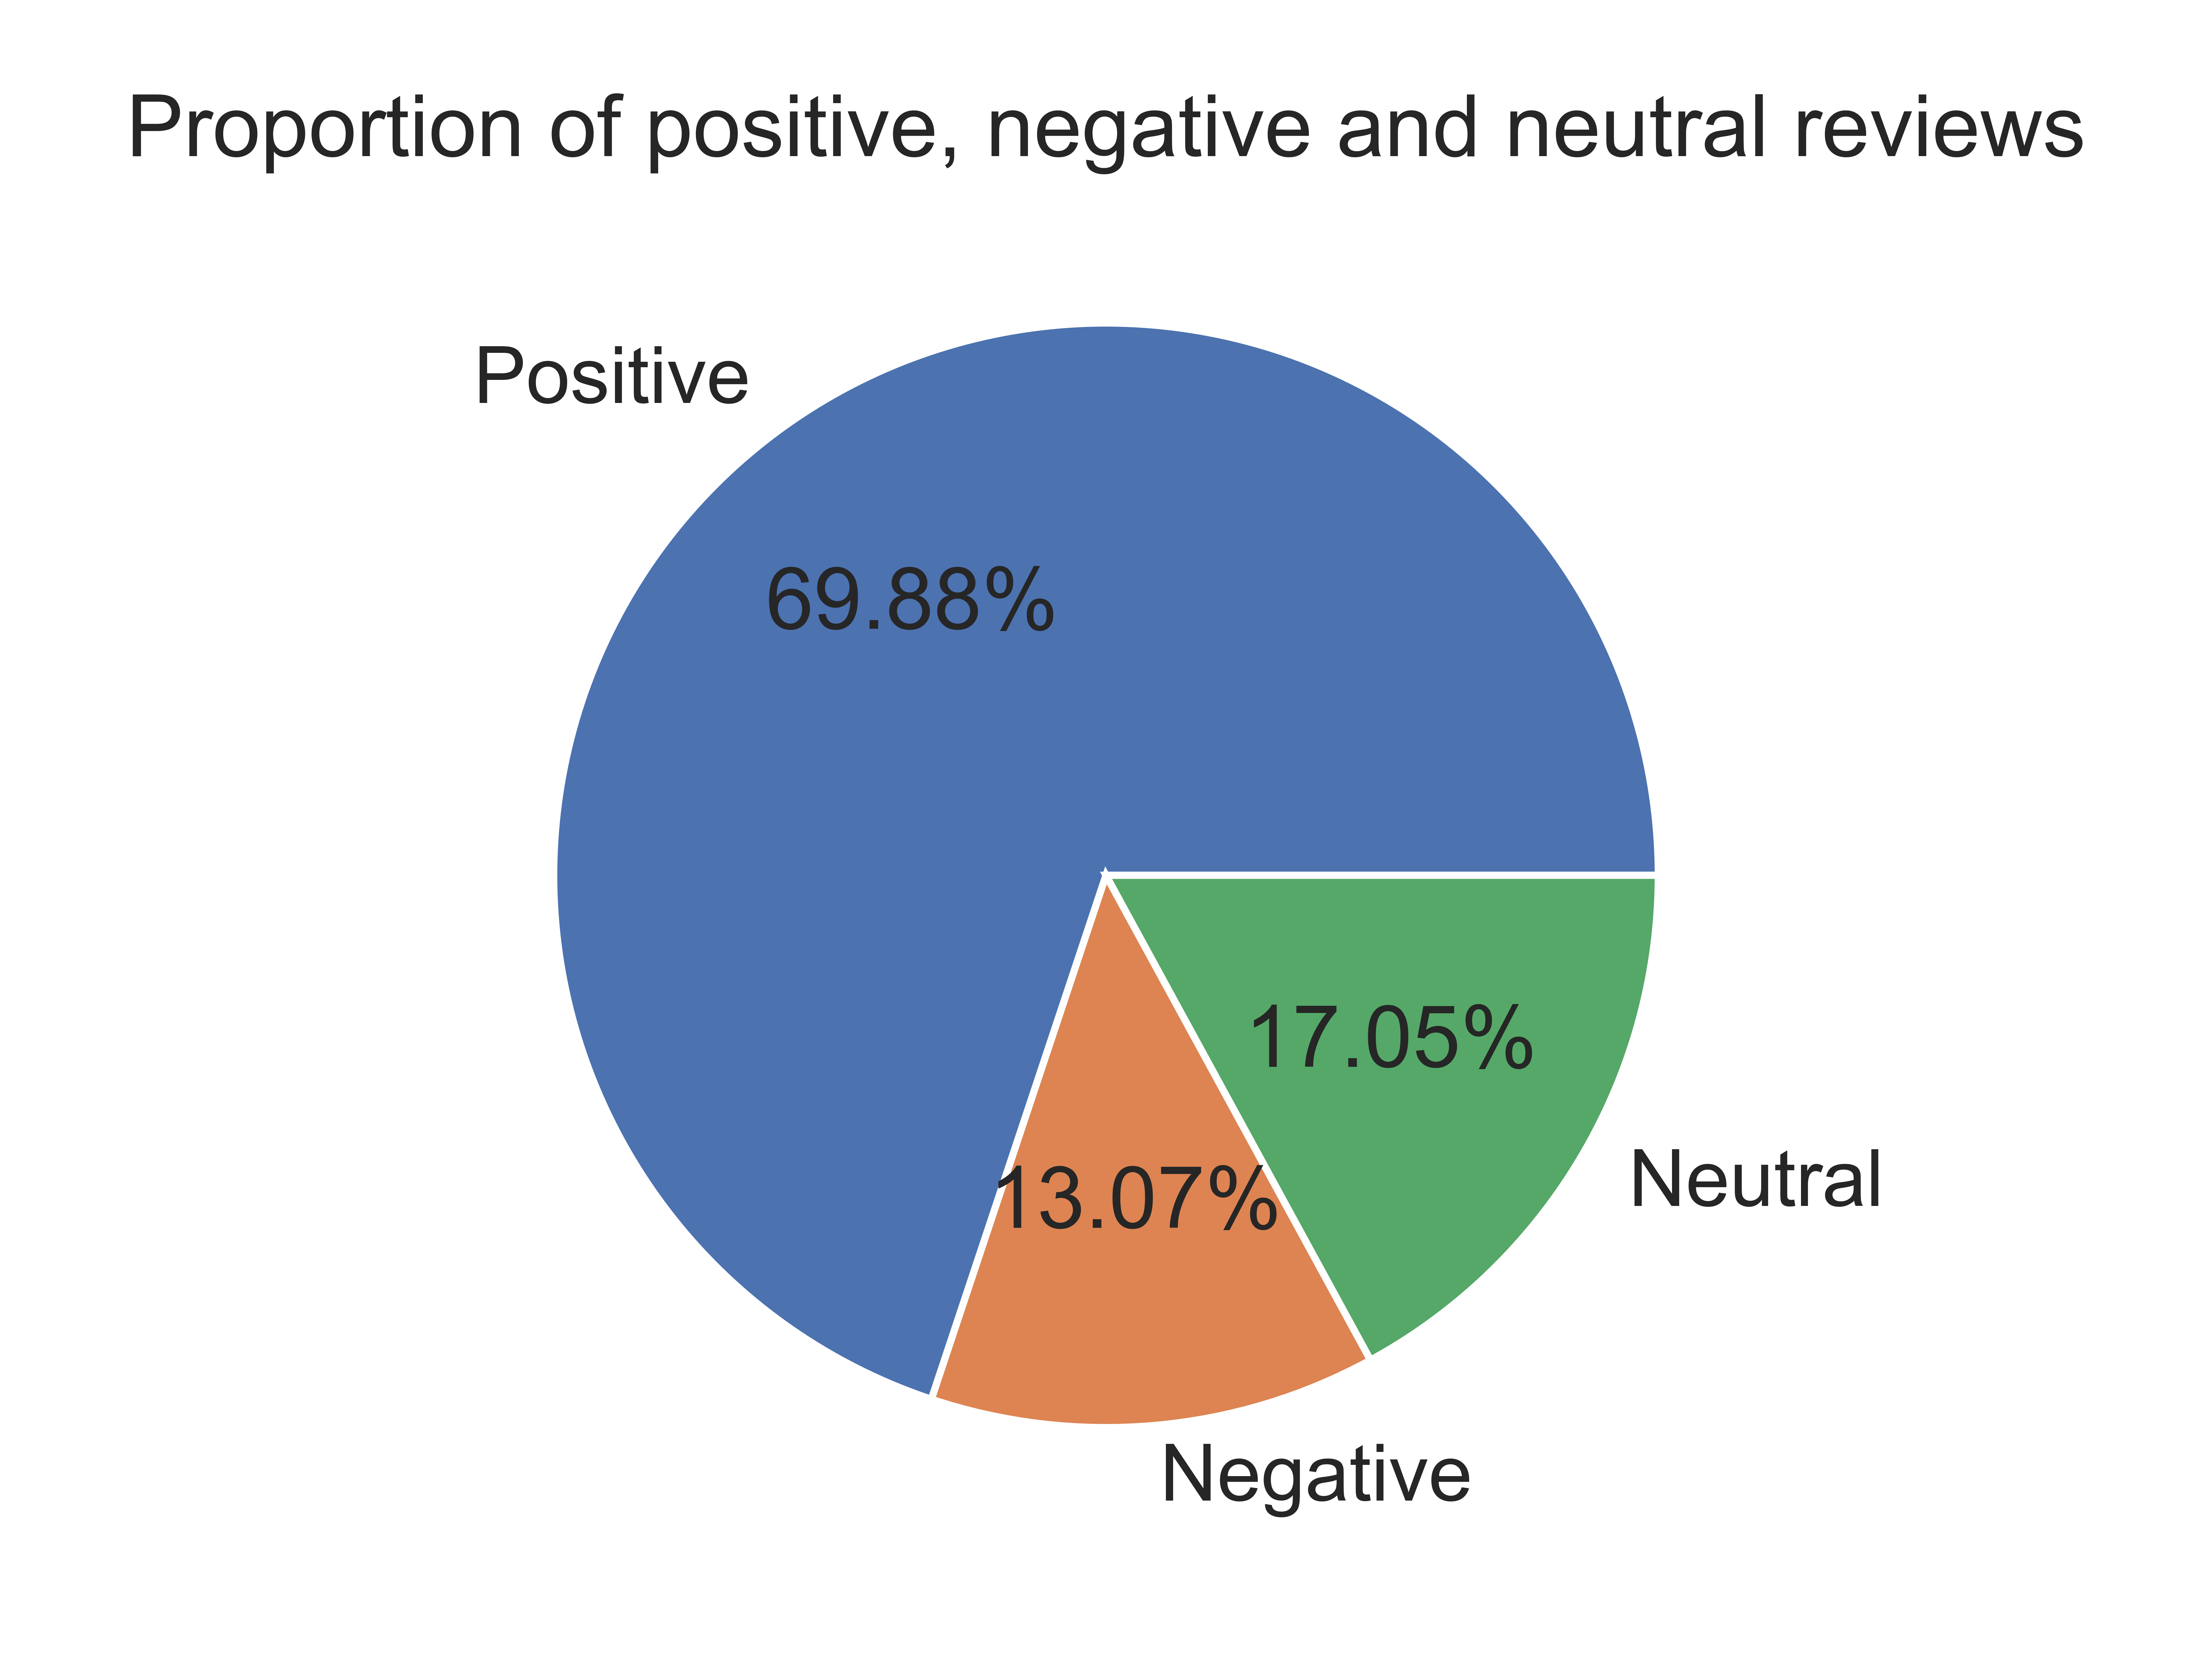
\includegraphics[width=0.9\textwidth]{../results/old/pie_tripartite.png}
		\caption*{Tripartite sentiment}
	\end{minipage}
	\caption{Proportion of reviews in dataset by polarity}
	\label{fig:pies}
\end{figure}

\subsection{Quantifying text}

A frequency table for all reviews was generated, showing how
often a review (with a overall score, \(s_+ + s_-\), between \(\left[-5, 5\right]\))
occurred in the dataset. Reviews of overall neutral score were also considered.
The results here are consistent with those earlier (Section~\ref{sec:reviews}),
where positive reviews of a moderate overall score made up the majority (Figure~\ref{fig:distribution}).

\begin{figure}[htpb]
	\centering
	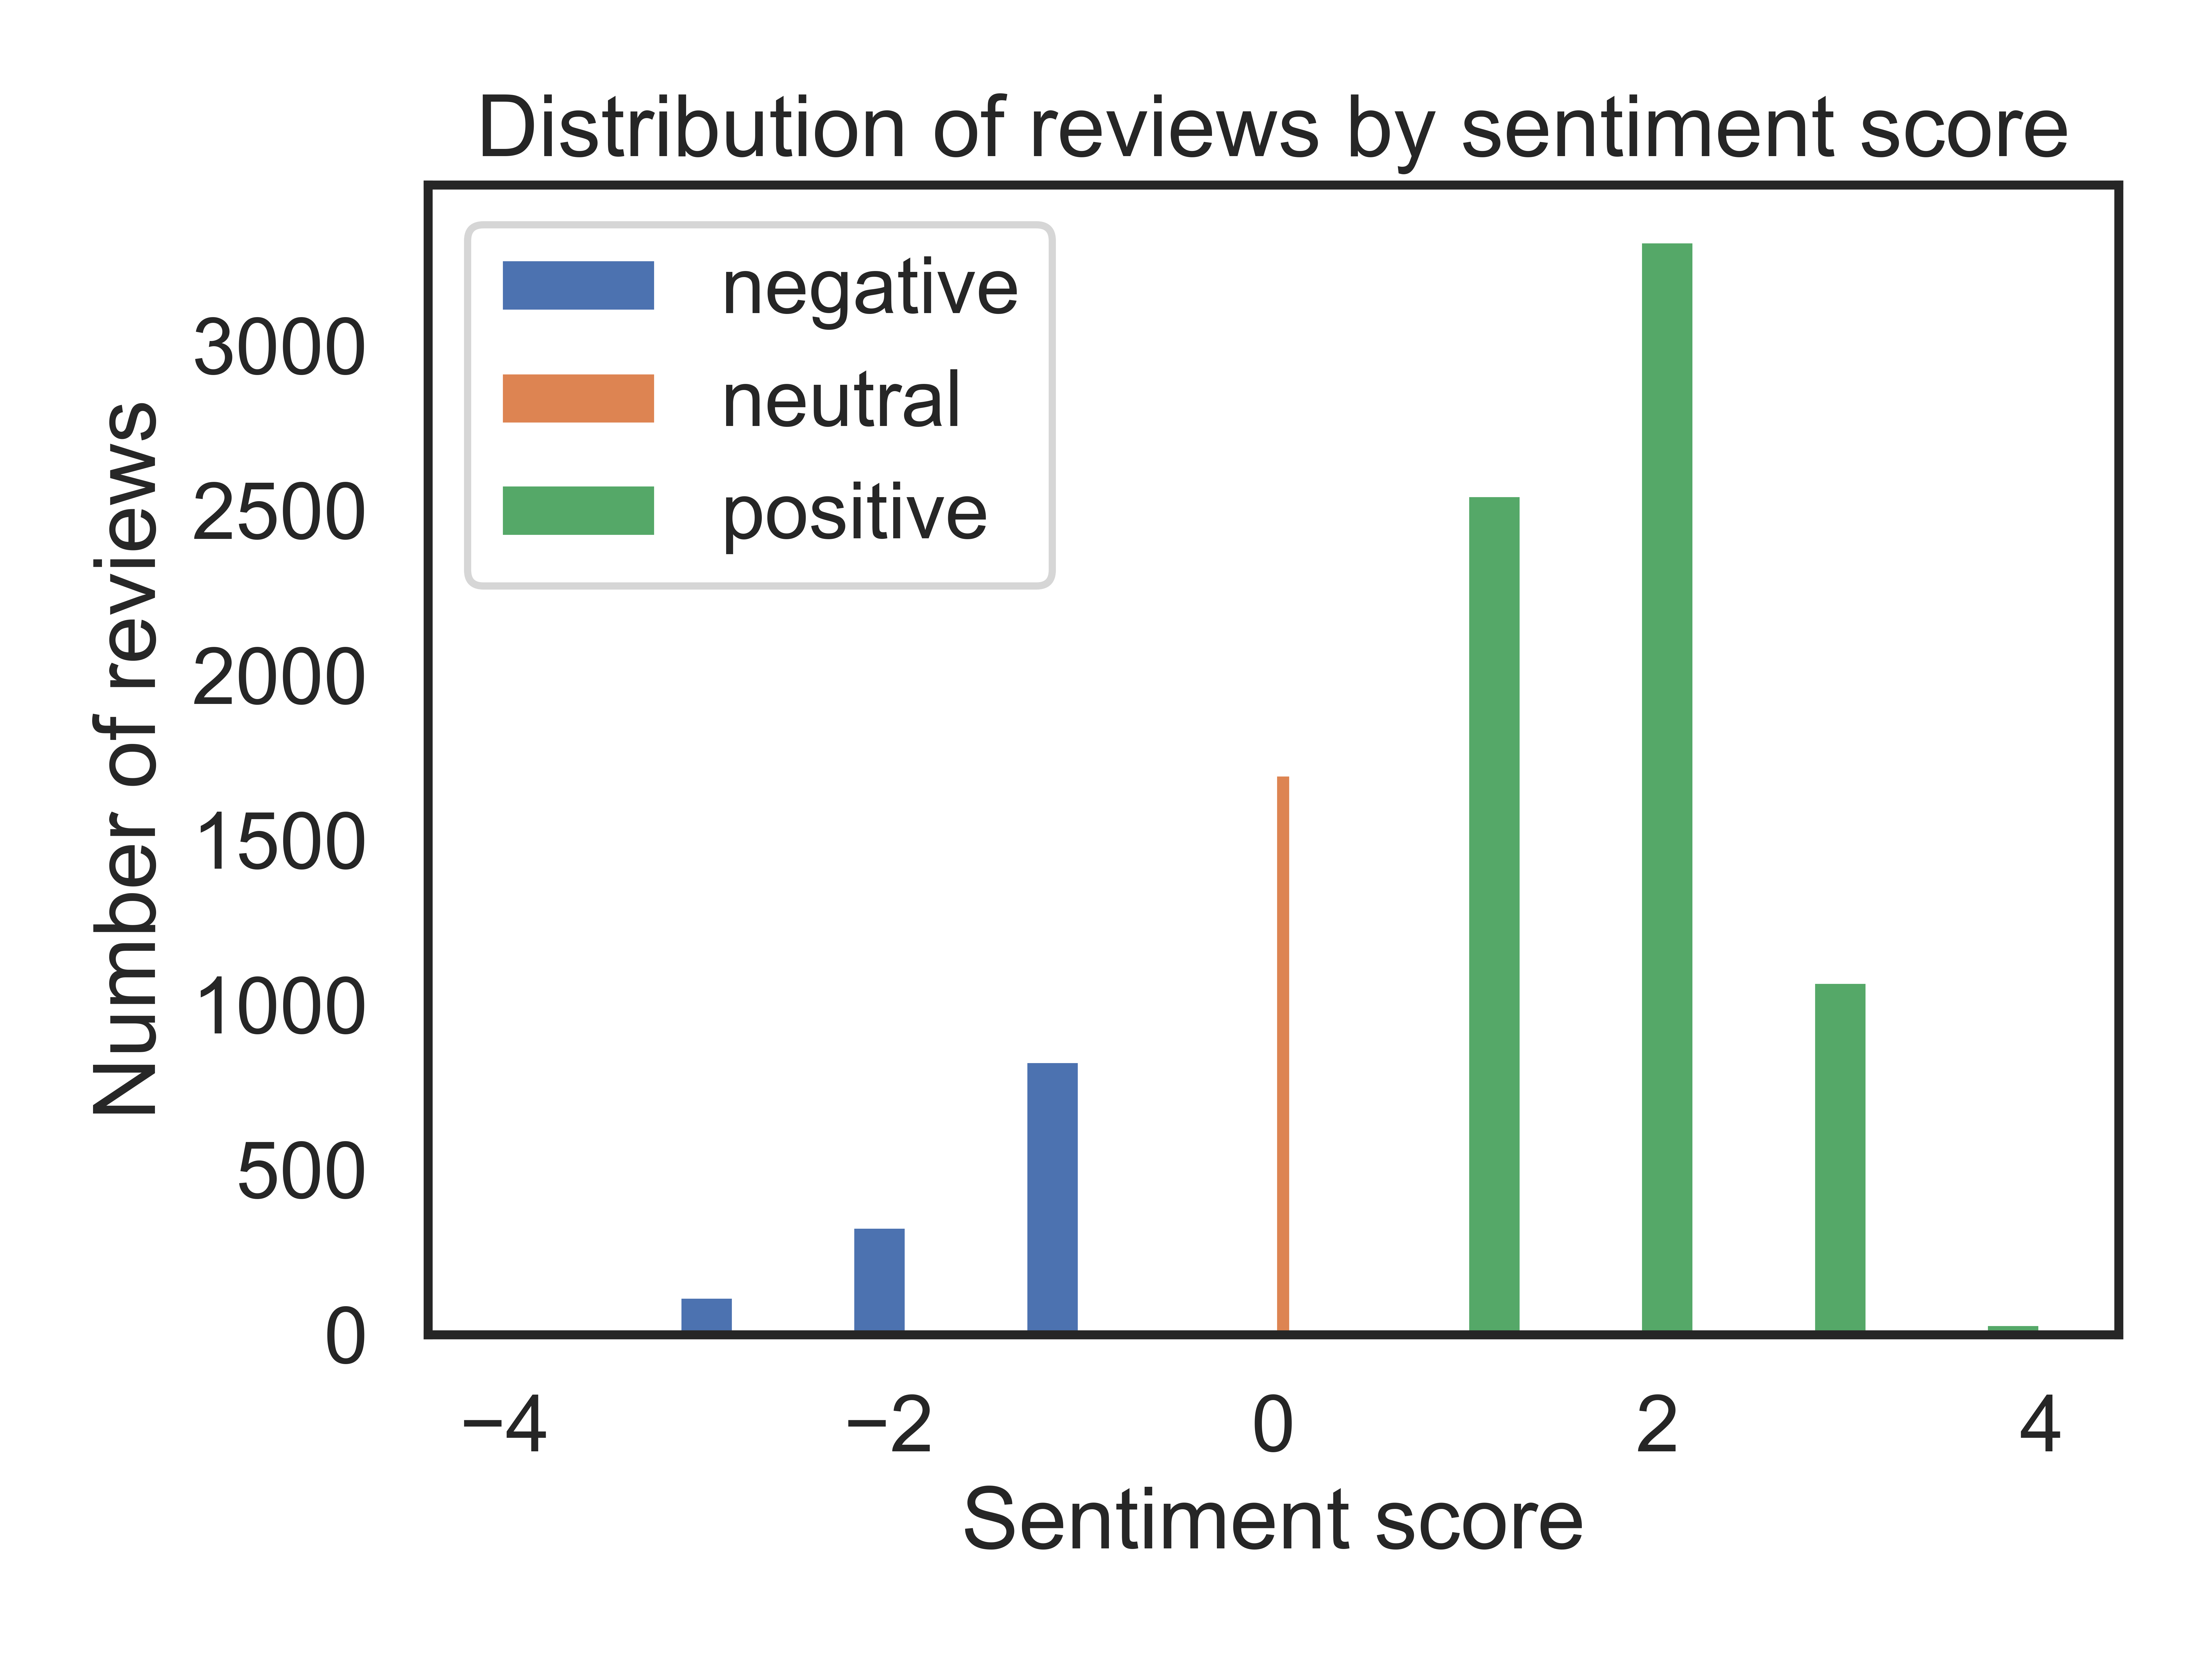
\includegraphics[width=0.75\textwidth]{../results/old/distribution.png}
	\caption{Distribution of reviews by sentiment score}
	\label{fig:distribution}
\end{figure}

For each review, a feature vector was constructed, which shows how
often each token in a review occurs within that review---the term frequency
of the token (Equation~\ref{eq:term-frequency}). \(\text{tf}\left(t, d\right)\)
represents the relative term frequency of token \(t\) in review (or \textit{document})
\(d\). \(f_{t, d}\) is the raw count of a token in a review.

\begin{equation}
	\text{tf}\left(t, d\right) = \frac{f_{t, d}}{\sum_{t' \in d}^{}f_{t',d}}
	\label{eq:term-frequency}
\end{equation}

It is noted that the denominator is simply the total number of tokens in document \(d\),
counting each occurrence of the same token separately.

To evaluate the relevance of a token \(t\) in determining the overall sentiment of the
review \(d\) in a corpus of reviews \(D\) of size \(N\), the term frequency-inverse document frequency
(tf--idf value) is found (Equation~\ref{eq:tf-idf}).

\begin{equation}
	\text{tfidf}\left(t, d, D\right) = \text{tf}\left(t, d\right)\log\frac{N}{1 + \left|\left\{d \in D : t\in d\right\}\right|}
	\label{eq:tf-idf}
\end{equation}

\(\left|\left\{d \in D : t \in d\right\}\right|\) is the number of reviews in which token \(t\) occurs.
Since the denominator will be \(0\) if the token does not appear in the review at all, \(1\) is added
to avoid a division-by-zero.

\subsection{Reducing bias using logistic regression}

Since the number of positive reviews greatly exceeds the number of negative reviews Figure~\ref{fig:pies},
the classification models trained would likely perform better at identifying positive reviews than their
negative counterparts. To counteract this, class weights for both the negative and positive classes of reviews
were found to ensure that positive and negative reviews receive equal emphasis during the training process.

A logistic regression model was constructed to maximise the $F_1$ score (Equation~\ref{eq:f1}) when
predicting the polarity of a review from its token frequencies.

\begin{equation}
	F_1 = \frac{2 T_p}{2 T_p + F_p + F_n}
	\label{eq:f1}
\end{equation}

where $T_p$ is the number of true positive predictions, $F_p$ is the number of false positive predictions,
and $F_n$ is the number of false negative predictions.

Each review's tf--idf values ($x$) were used as the independent variable and the polarity of a review ($y$) was set
as the dependent variable. A conventional sigmoid function was used to evaluate the probability of a review being positive, in the range
\(\left(0, 1\right)\) (Equation~\ref{eq:sigmoid}), where \(x_i\) is the tf--idf value of token \(t_i\) in
review \(d_i\):

\begin{equation}
	h\left(x_i\right)	= \frac{1}{1 + e^{-\left(\beta_0 + \beta_1 x_i\right)}}
	\label{eq:sigmoid}
\end{equation}

Here, \(\beta_0 + \beta_1 x_i\) is an arbitrary linear function of tf--idf \(x_i\), chosen
such that the loss, \(l_i\), is minimised. Let \(y_i\) be the actual polarity of review \(i\),
determined through Equation~\ref{eq:polarity}.

The loss, \(l_i\), for the \(i\)-th tf--idf value is given as (Equation~\ref{eq:logloss}):
\begin{equation}
	l_i = \frac{1}{N} \sum^{N}_{i = 1}\left[-w_0 y_i \log h_i + w_1\left(1 - y_i\right) \log \left(1 - h_i\right)\right]
	\label{eq:logloss}
\end{equation}

The loss measures how ``surprising'' the outcome ($y_i$) is to the predicted
value ($h_i$); perfect predictions warrant a loss of $0$. We define $w_0$ and $w_1$
to be the class weights for the negative ($0$) and positive ($1$) review classes
respectively.

It was determined that $w_1 \approx 0.44$ was the most optimal positive class weight (Figure~\ref{fig:f1-variation}).
$w_0$ was set to $1 - w_1 \approx 0.56$.

\begin{figure}
	\begin{center}
		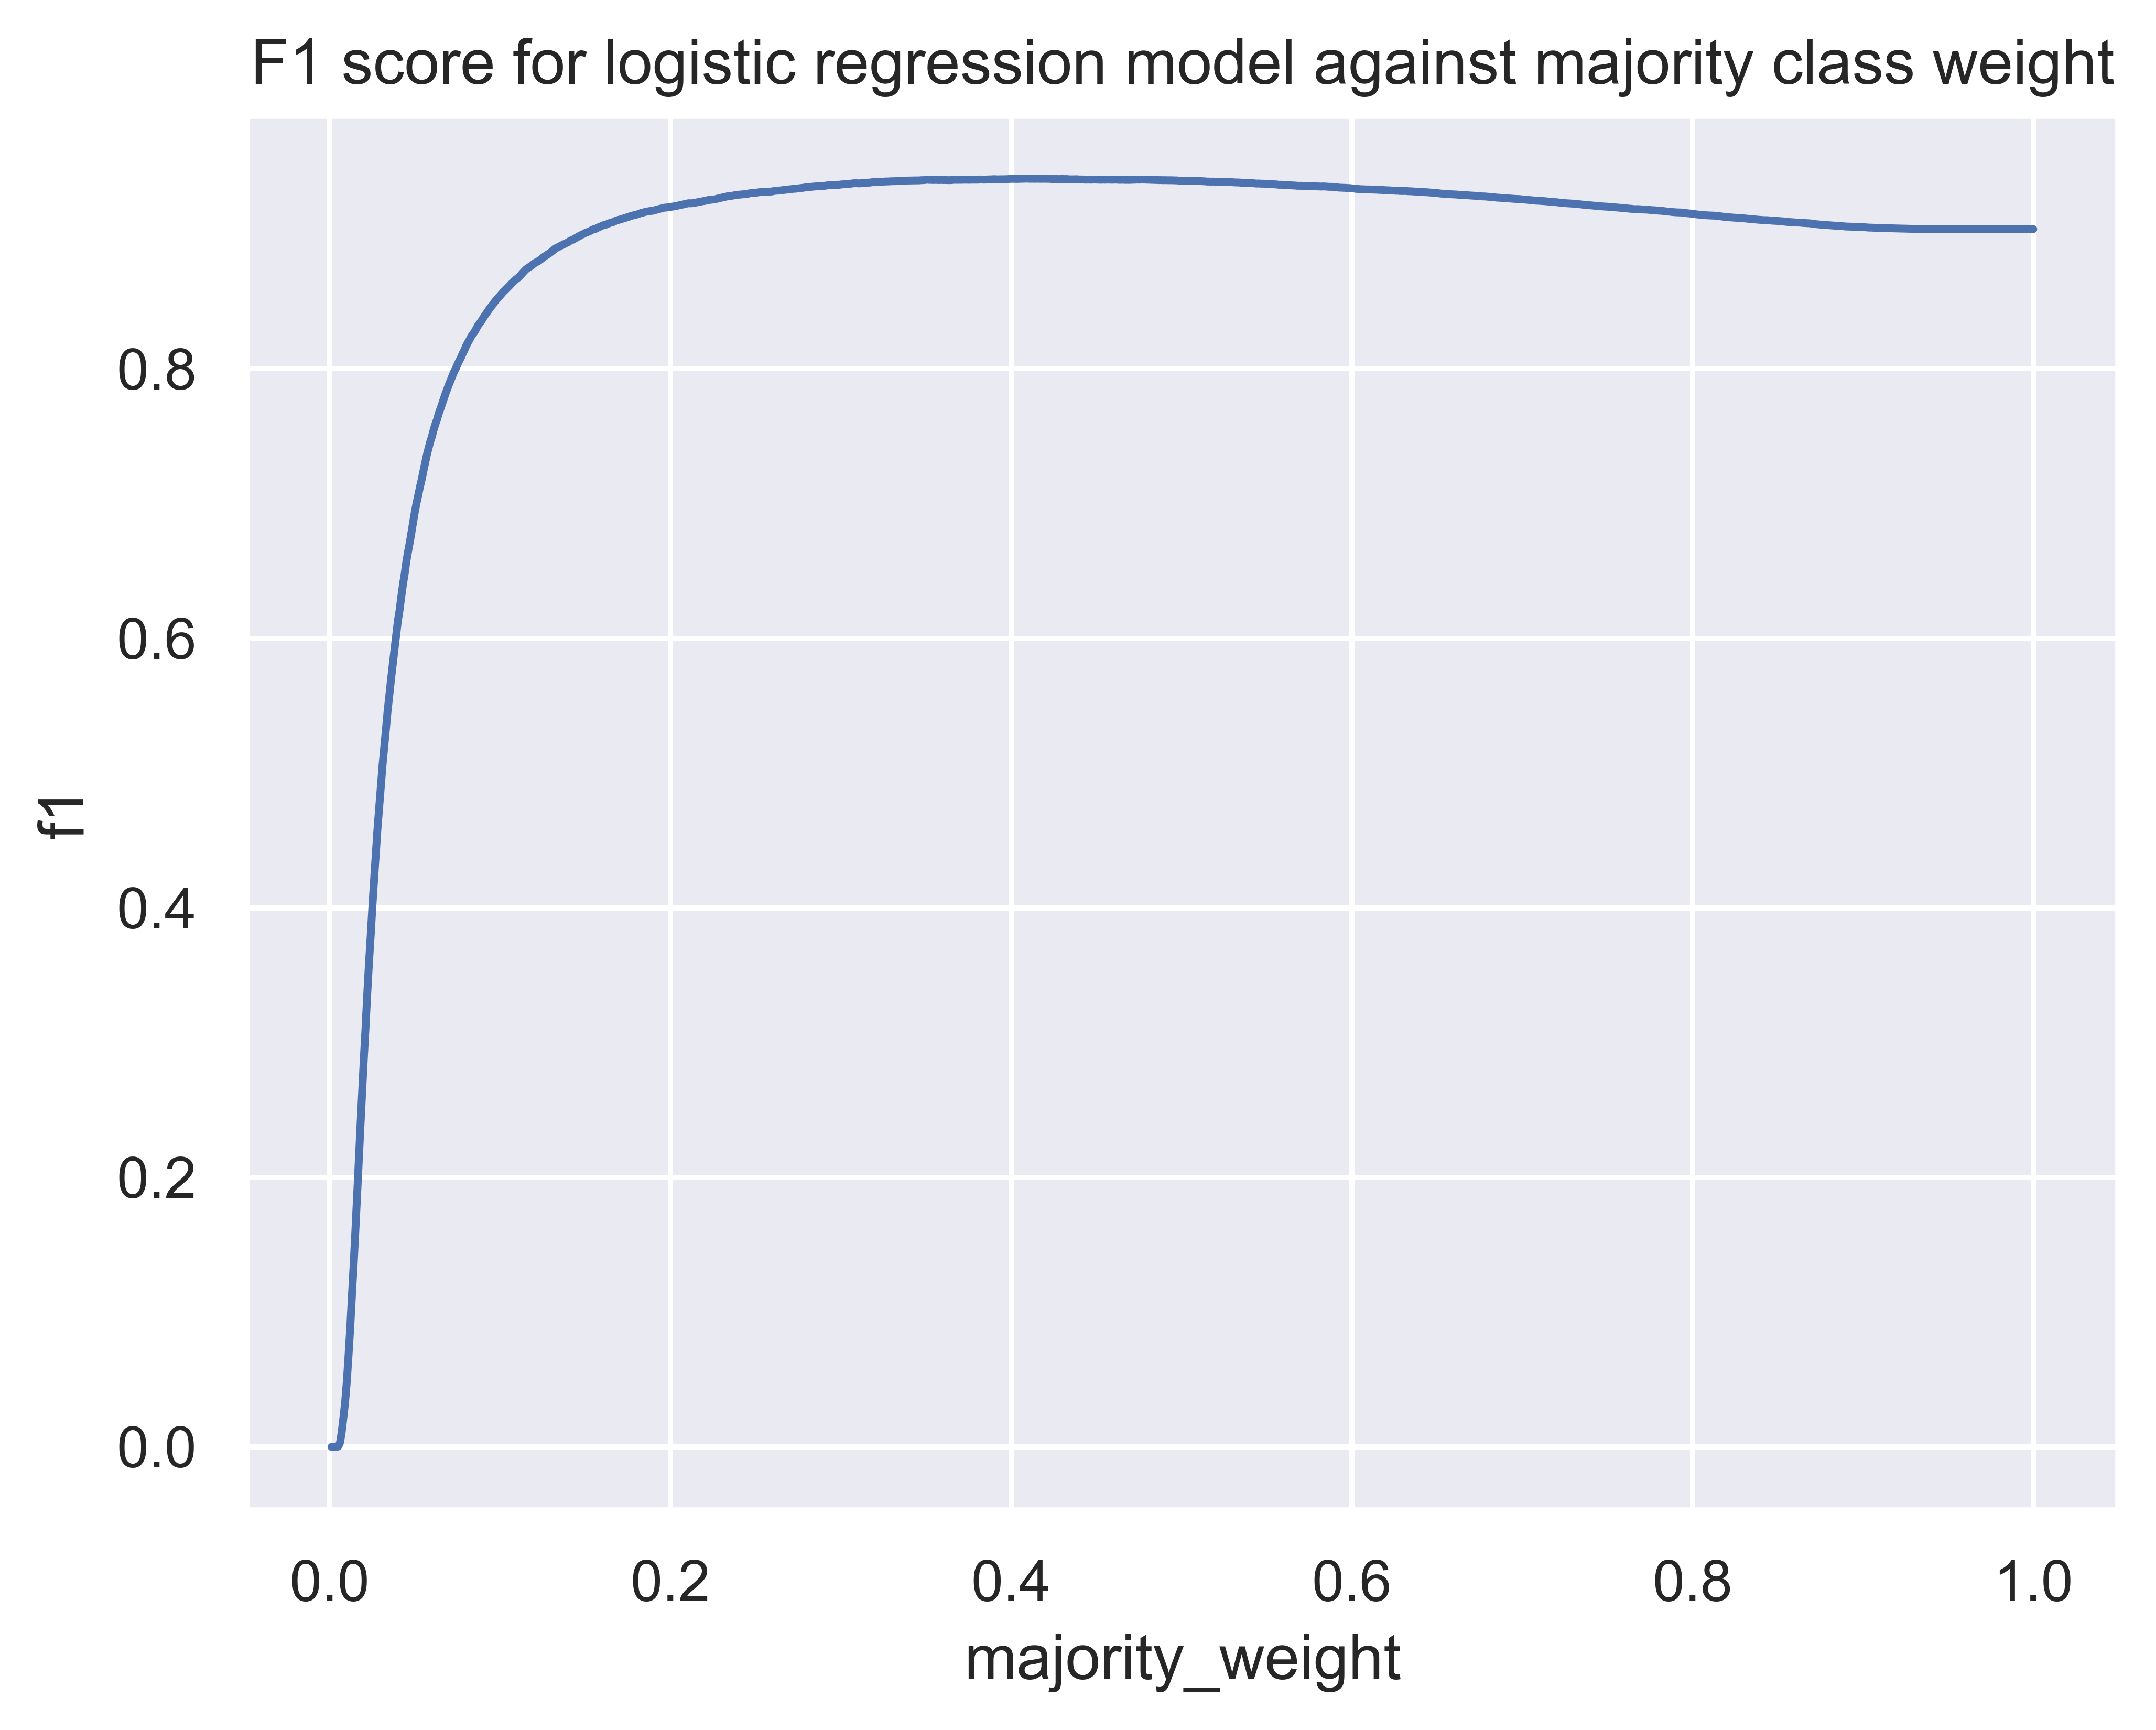
\includegraphics[width=0.75\textwidth]{../results/logistic_f1.png}
	\end{center}
	\caption{Variation of $F_1$ score against positive class weight}\label{fig:f1-variation}
\end{figure}

A confusion matrix was used to evaluate the performance of the logistic regression model. In
four quadrants, the confusion matrix shows the relative proportions of $T_p$, $T_n$ (true negative
predictions), $F_p$ and $F_n$. Higher proportions of $T_p$ and $T_n$ indicate that the model performs
better at making predictions.

\begin{figure}
	\begin{center}
		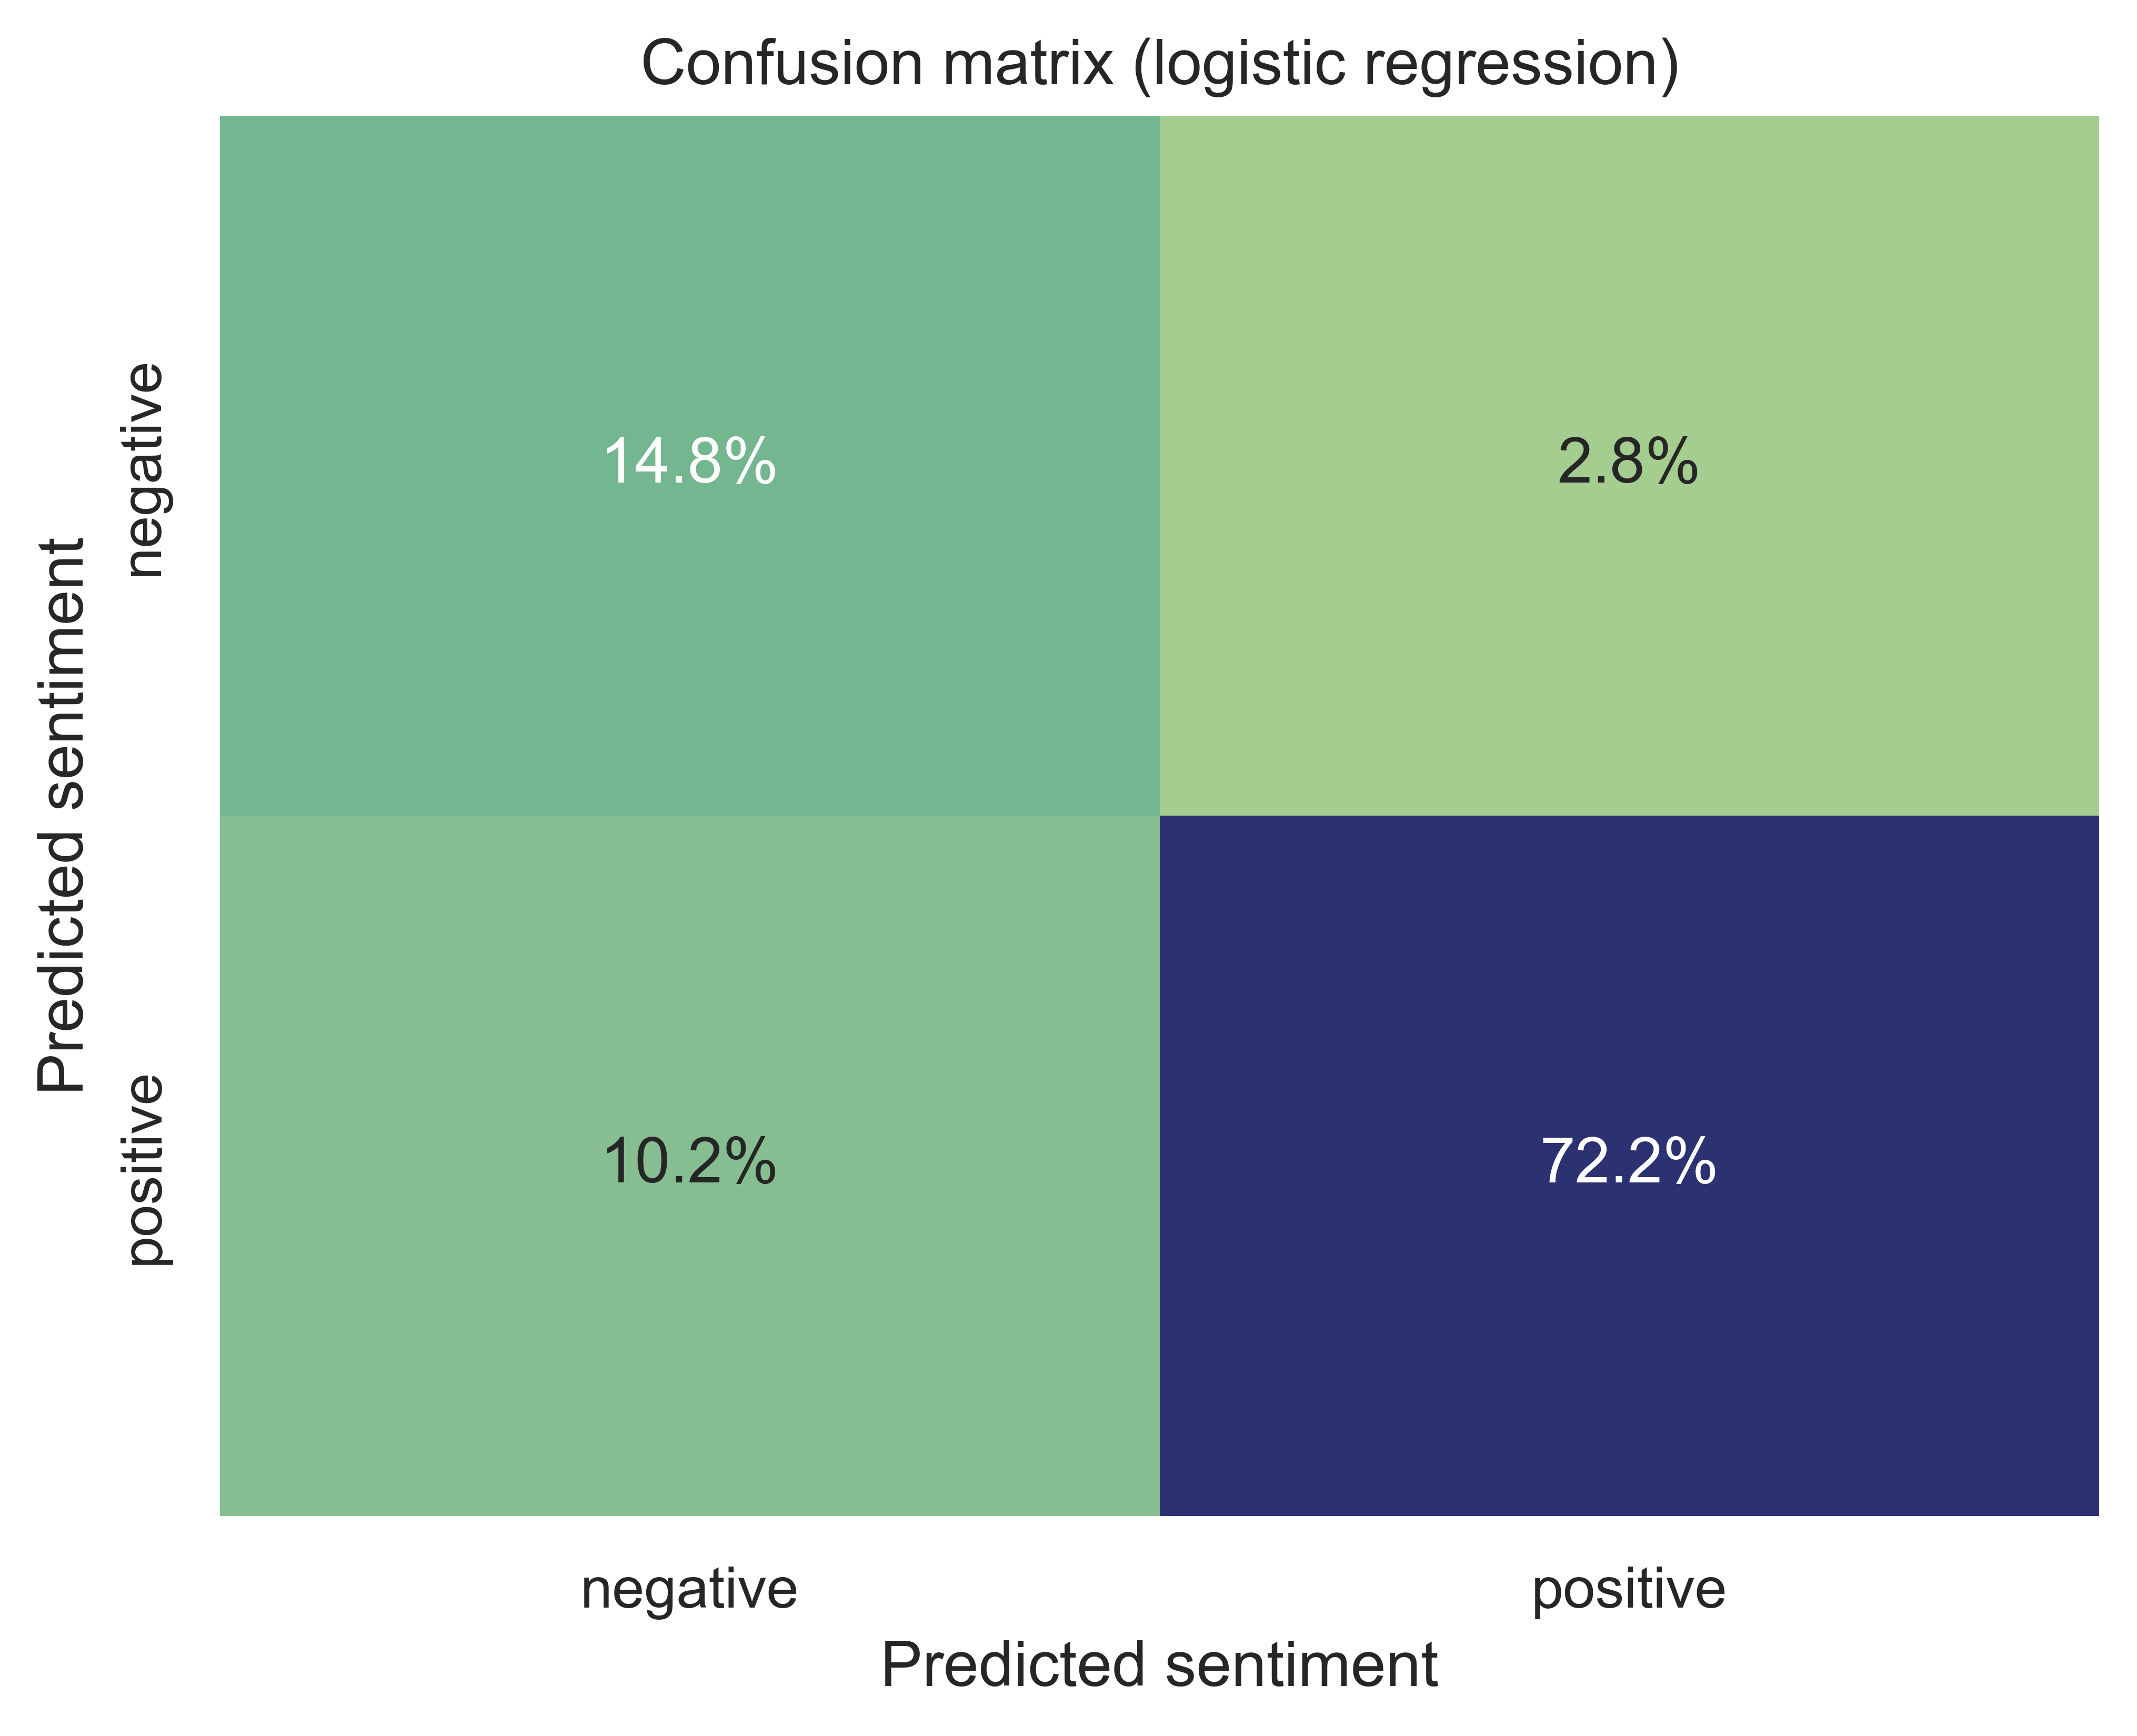
\includegraphics[width=0.75\textwidth]{../results/logistic_confuse.png}
	\end{center}
	\caption{Confusion matrix (logistic regression model)}\label{fig:logistic-confuse}
\end{figure}

Figure~\ref{fig:logistic-confuse} indicates that $\qty{72}{\percent}$ of reviews were correctly predicted as positive, a large proportion.
Furthermore, the proportion of incorrect predictions---false negatives and false positives, only made up
$\qty{13}{\percent}$ of the entire set of predictions. Therefore, the logistic regression model performs
well at reducing bias.

\subsection{Predicting review polarity from token frequency}

A large variety of classification models were constructed to make predictions using the aforementioned
dataset of hotel reviews. These include:

\begin{itemize}
  \item a \textit{random forest classifier} (\texttt{RandomForestClassifier}), which makes predictions based on the average of the results from multiple decision trees,
  \item a regularised linear model with \textit{stochastic gradient descent} (\texttt{SGDClassifier}): the gradient of the loss function is estimated one review at a time and the model's learning rate is updated accordingly,
  \item a $k$-\textit{nearest neighbours} algorithm (\texttt{KNeighborsClassifier}), which predicts the polarities of new reviews based on its proximity to other reviews' tf--idf vectors in vector space,
  \item a \textit{naive Bayes classifier} (\texttt{BernoulliNB}), which uses the rule in Equation~\ref{eq:nb} to make predictions, and
  \item $K$-\textit{means clustering} (\texttt{KMeans}), which unsupervisedly classifies tf--idf vectors into two classes such that each vector belongs to the cluster with the mean of that cluster being the closest to it.
\end{itemize}

\begin{equation}
  P\left(x_i|y \right) = P\left(x_i = 1 | y\right)x_i + \left(1 - x_i\right)\left[1 - P\left(x_i=1|y\right)\right]
  \label{eq:nb}
\end{equation}

Their performances were evaluated using three metrics: $F_1$ score, the area under receiver operating characteristic
curve (AUROC) and their average precisions (Table~\ref{tab:metrics}).

\begin{table}
	\centering
	\caption{Performance metrics for classification models}
	\label{tab:metrics}
	\begin{tabular}{lrrr}
		\toprule
		\textbf{Model} & $F_1$ & AUROC & Avg. precision \\
		\midrule
		\csvreader[head to column names, late after line=\\]{../results/model_metrics_27032024.csv}{
			name=\name,
			f1=\fone,
			auroc=\auroc,
			averageprecision=\avgprecision
		}{\texttt{\name} & \fone & \auroc & \averageprecision}
		\bottomrule
	\end{tabular}
\end{table}

It is shown that all constructed models performed well in all three metrics, being
able to make true positive predictions much of the time, distinguish true and false
positive predictions with great success and return relevant results. Notably, the KMeans
model performs the worst out of all models: due to the unsupervised nature of the prediction
model, the target class of each review (either negative or positive) was not revealed to it,
leading it to make more incorrect predictions.

The receiver operating characteristic curves (ROC) (Figure~\ref{fig:roc-all}) and precision-recall curves (PRC)
(Figure~\ref{fig:prc-all}) of each model were plotted to better examine the latter two metrics.

The receiver operating characteristic curve (ROC) plots the rate of true positive predictions ($\text{TPR}$) made against the
rate of false positive predictions ($\text{FPR}$) made. A model's ability to distinguish
true positive and false positive predictions may be inferred from the height at which the ROC curve
lies over that of a hypothetical classifier which chooses each outcome randomly. It is noted that
the KMeans algorithm's ROC curve lies below the baseline denoted by the random classifier.
Due to the absence of target classes during the training process, it falls short in distinguishing
true and false positive predictions reliably. Other models perform significantly better in this aspect.

\begin{figure}
  \begin{center}
    \includegraphics[width=0.95\textwidth]{../results/all_roc.png}
  \end{center}
  \caption{Receiver operating characteristic curves for all models}\label{fig:roc-all}
\end{figure}

The precision-recall curve (PRC) plots a model's precision ($p$, Equation~\ref{eq:precision})
against its recall ($r$, Equation~\ref{eq:recall}). A high area under the curve represents both high recall and high precision, where high precision relates to a low false positive rate, and high recall relates to a low false negative rate. High scores for both show that the classifier is returning accurate results (high precision), as well as returning a majority of all positive results (high recall). It is noted that all models perform well in this regard,
except the KMeans algorithm, for similar reasons as above.

\begin{equation}
  p = \frac{T_p}{T_p + F_p}
  \label{eq:precision}
\end{equation}

\begin{equation}
  r = \frac{T_p}{T_p + F_n} 
  \label{eq:recall}
\end{equation}

\begin{figure}
  \begin{center}
    \includegraphics[width=0.95\textwidth]{../results/all_prc.png}
  \end{center}
  \caption{Precision-recall curves for all models}\label{fig:prc-all}
\end{figure}

\section{Conclusion}

\subsection{Summary}

Sentiment analysis was performed on a dataset of international hotel reviews
in English. Hotel reviews were tokenised---split into individual words which
carry tangible meaning---and their sentiments were determined using a sentiment
lexicon. Although the majority of the lexicon contained neutral tokens,
such as \textit{hotel}, \textit{visit} and \textit{food}, the number of tokens
that carry positive sentiment far exceeds that with negative sentiment.

On a larger scale, the sentiments of individual hotel reviews were quantified
using SentiStrength, with positive reviews greatly outnumbering negative ones
by a considerable margin.

Multiple classification models were trained to
predict the sentiments of hotel reviews. Upon making predictions, the models
were found to have moderately high average precisions and high rates of
success in distinguishing false and true positive predictions. This was
in part due to the integration of class weights into the training process,
which reduced model bias.

\subsection{Limitations}

Homographs---words that have the same spelling but different meanings---could
not be distinguished during tokenisation (Section~\ref{sec:tokens}), resulting in
slightly unreliable sentiment scores. For instance, the word \textit{lobby} was shown to
carry a negative sentiment (Figure~\ref{fig:wordclouds}). However, the word \textit{lobby}
was only used to refer to a hotel lobby upon closer inspection.

Furthermore, the data collected was limited only to English international hotel reviews.
A more complete analysis of hotel reviews would include tourists of different language
backgrounds; hence, sentiment analysis would need to be conducted in more than one language.

A logistic regression model, used to determine the optimal class weights, assumes that the tf--idf values of tokens
and the overall sentiment of a review are linearly related (because of the linear component $\beta_0 + \beta_1x_i$
in Equation~\ref{eq:sigmoid}), which may hinder the accuracy of the predictions it makes.

\subsection{Future work}

Much can be done to extend this project, because of the relatively small scale on which this project
was conducted. As above, sentiment analysis could be conducted in more than one language (besides English)
to gain a broader understanding of tourists' preferences in hotels from different languages and cultural
backgrounds.

Furthermore, more prediction models could be constructed. This would create a larger
variation in the predictions made, enabling the precision of the models used in this project to be
compared with those of other models to evaluate the model with the highest accuracy. Constructing a
wider range of prediction models also allows for the possibility of more advanced techniques,
including recurrent neural networks, which are
widely used in analysing sentiment from textual data. In particular, recurrent neural
networks perform better at analysing tokens in context, avoiding the issue
of unreliable sentiment scores described above.

\pagebreak
\printbibliography[heading=bibintoc]

\end{document}
